%------------------
% General Settings
%------------------
\def \docTitle      {Data sheet}
\def \docSubTitle   {SMCx242}
\def \productNumber {SMCx242}
\def \productName   {Stepper Motor Controller}
\def \docAuthor     {LK-Instruments}
\def \docRevision   {Rev. 001}
\def \docSubject    {\docAuthor \docTitle \docSubTitle}
\def \docKeywords   {\docAuthor, \productName, \productNumber, SMC2242, SMC4242}

\documentclass[a4paper, final, 12pt, oneside]{scrartcl}

%----------
% Packages
%----------
\usepackage{etex}
\reserveinserts{30}
\usepackage[utf8]{inputenc}
%\usepackage[latin1]{inputenc} % erlaubt Umlaute in der tex-Datei

\usepackage{slantsc}
\usepackage[urw-garamond]{mathdesign}
\usepackage{garamondx}
\usepackage[T1]{fontenc}

\usepackage[english]{babel}              % For the hyphenations in different languages
\usepackage[intlimits]{amsmath}          % math symbols
\usepackage{braket}                      % Dirac braket notation
\usepackage{graphicx}                    % include pictures
\usepackage{color}
%\usepackage[shell]{gnuplottex}           % gnuplot in latex
\usepackage{pstricks}                    % post script tricks
\usepackage{listings}                    % enter programming code
\usepackage{fancyhdr}                    % make quite nice header/footer
%\usepackage[version=3]{mhchem}           % chemistry stuff
\usepackage{relsize}
\usepackage{afterpage}
\usepackage{gensymb}
\usepackage{textcomp}
\usepackage{multicol}
%\usepackage{subfig}
\usepackage{lipsum}
\usepackage{multirow,booktabs,colortbl,tabularx}
\usepackage{caption}
\usepackage{subcaption}


\usepackage{pgfplots}
\usepackage{tikz}                        % beautiful plots
\pgfplotsset{compat = newest}
\usepackage{units}                       % easy to use number-unit-package
\usepackage[section]{placeins}           % Float barrier for sections.

\usetikzlibrary{trees,positioning}

\usepackage{listings}					% erlaubt Quellcode mit Zeilenumbruechen

%----------------
% PDF properties
%----------------
\usepackage[
  pdftitle={\docAuthor~\docSubTitle~\docTitle}
 ,pdfsubject={\docSubject}
 ,pdfauthor={\docAuthor}
 ,pdfkeywords={\docKeywords}
 ,pdfcreator={\docAuthor}
 ,pdfstartview=Fit                       % startseite ganz anzeigen
 ,pdfborder={0 0 0}                      % links ohne umrandungen
 ,pdfdisplaydoctitle=true                % pdftitle statt dateinamen anzeigen
 ,pdfcenterwindow=true                   % position pdf in center of the screen
 ,setpagesize=true
]{hyperref}

%-------------------
% Header und Footer
%-------------------
\fancyhf{}        % clear all header/footer
\renewcommand{\headrulewidth}{0pt}
%\renewcommand{\sectionmark}[1]{\markboth{#1}{}}
%\renewcommand{\subsectionmark}[1]{\markright{#1}}
\fancyhead[RE,RO]{\productNumber}
\fancyfoot[LE,LO]{\docAuthor}
\fancyfoot[CE,CO]{\docRevision}
\fancyfoot[RE,RO]{\thepage}

\pagestyle{fancy}

% number equations with sections before equation-index
\numberwithin{equation}{section}
\numberwithin{table}{section}
\numberwithin{figure}{section}

%---------------------
% My code definitions
%---------------------

\newtheorem{envdefinition}{Definition}[section]
\newtheorem{envsatz}{Satz}

% special numbers and letters
\renewcommand{\i}{\mathrm{i}}                  % complex i
\newcommand{\e}{\mathrm{e}}                    % Eulers number
\renewcommand{\phi}{\varphi}                   % nicer phi
\renewcommand{\epsilon}{\varepsilon}           % nicer epsilon
\renewcommand{\theta}{\vartheta}               % nicer theta
\renewcommand{\rho}{\varrho}                   % nicer rho
%\newcommand{\degree}{^{\circ}}                 % degree-circle

% vectors and matrices
\renewcommand{\vec}[1]{\boldsymbol{#1}}
\newcommand{\Vek}[3]{\left(\begin{array}{c}#1\\#2 
\ifthenelse{\equal{#3}{}}{}{\\#3}\end{array}\right)}

% integral and derivative stuff:
\renewcommand{\d}[1]{\;\mathrm{d}#1}           % integeration d
% total derivative
\newcommand{\td}[1]{\frac{\mathrm{d}}{\mathrm{d}#1}\,}
\newcommand{\pd}[1]{\partial_{#1}\,}             % partial derivative

% Braket notation
\renewcommand{\bra}{\Bra}
\renewcommand{\ket}{\Ket}
\renewcommand{\braket}{\Braket}
\renewcommand{\set}{\Set}

% plus-minus with braces
\newcommand{\PM}{\ensuremath{\substack{+\\[-0.25em]-}\,}}
\renewcommand{\pm}{\PM}
\newcommand{\pmp}{\ensuremath{\substack{\mathsmaller{(}+\mathsmaller{)}\\[-0.25em]-}\,}}
\newcommand{\pmm}{\ensuremath{\substack{+\\[-0.25em]\mathsmaller{(}-\mathsmaller{)}}\,}}

\setlength{\columnsep}{40.0pt}

%----------------------------------------------------------
% let the party start
%----------------------------------------------------------
\begin{document}
\thispagestyle{empty}

\begin{minipage}{\textwidth}
  \begin{minipage}[h]{0.125\textwidth}
      
\includegraphics[width=1\textwidth]{../general/logo_black.pdf}
  \end{minipage}
  \hfill
  \begin{minipage}[h]{0.8\textwidth}
      {\huge \textbf{\textsf{\productName}}}\\
      {\huge \textbf{\textsf{\productNumber}}}
  \end{minipage}
\end{minipage}       
       
\vspace*{5pt}
\rule{\textwidth}{0.4pt}

\begin{multicols}{2}
\subsection*{Features}
\begin{itemize}
  \item Intuitive manual user interface
  \item Well readable OLED display
  \item Fully-featured remote interface
  \item Automatic motor detection
  \item Automatic position calibration
  \item Up to \unit[2.5]{A} of output current
  \item 24 V operating voltage
  \item Up to 1/32 microstepping
  \item Up to three limit/home switches per channel
\end{itemize}
\FloatBarrier

\subsection*{Applications}
\begin{itemize}
  \item[] Polarization adjustment
  \item[] Grating positioning
  \item[] Neutral density filter positioning
\end{itemize}
\FloatBarrier

\subsection*{Description}
The LK-Instruments SMC2242/SMC4242 is a universal Stepper Motor Controller for two/four bipolar stepper motors. It offers a  comfortable manual user interface as well as fully-featured remote interface via a virtual COM port. This allows for simultaneous remote and manual control over stepper motor driven systems.
\end{multicols}
\noindent\rule{\textwidth}{0.4pt}
\vspace*{0.5cm}

\centerline{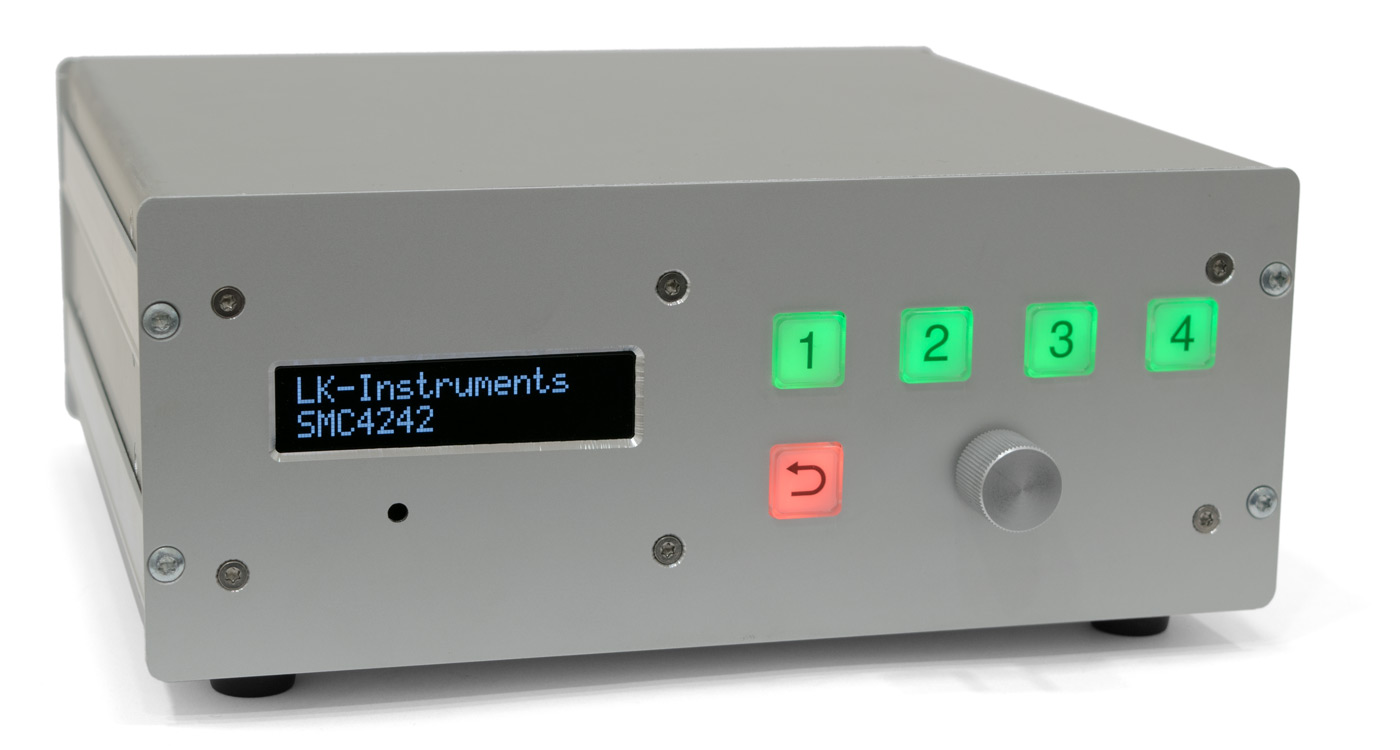
\includegraphics[width=0.7\textwidth]{./drawings/SMC_1400.jpg}}

\vfill
\begin{minipage}{\textwidth}
  \begin{minipage}[t]{0.49\textwidth}
      
    
  \end{minipage}
  \hfill
  \begin{minipage}[t]{0.49\textwidth}
    \begin{flushright}
    {\footnotesize LK-Instruments\\
             Welzheimer Str. 49\\
             71554 Weissach im Tal\\
             Germany\\
             \href{http://www.lk-instruments.com}{www.lk-instruments.com}}
    \end{flushright}
  \end{minipage}
\end{minipage}






\FloatBarrier

\newpage
\subsection*{Specifications}
$T_A = \unit[25]{^{\circ}C}$ and 50\% RH unless otherwise noted.
\newcolumntype{C}[1]{>{\centering\arraybackslash}p{#1}}
\begin{table}[!htp]
  \centering
  \begin{tabular}{C{2cm} C{2cm} *{3}{C{1cm}} *{3}{C{1cm}} C{1.5cm} }
    \toprule
    \textbf{Parameter} & \textbf{Conditions} &
    \multicolumn{3}{p{3cm}}{\centering\textbf{SMC2242}} &
    \multicolumn{3}{p{3cm}}{\centering\textbf{SMC4242}} &
    \textbf{Unit} \\
    \cmidrule(lr){3-5} \cmidrule(lr){6-8}
    & &
    Min & Typ & Max &
    Min & Typ & Max &\\
    \toprule
    Current &  & 0 & & 2.5 & 0 & & 2.5 & A/Phase\\ \midrule
    Gear ratio &  & & & & & & &  \\ \midrule
    Temperature range &  & 0 &  & 40 & 0 &  & 40 & $^{\circ}$C \\ \midrule
    Weight &  & & ??? & & & ??? & & kg \\ \midrule
    Operating voltage &  & & 24 & 36 & & 24 & 36 & VDC \\ \midrule
    Power consumption &  & & ??? & ??? & & ??? & ??? & W \\
    \bottomrule
  \end{tabular}
\end{table}
\vfill

\FloatBarrier
\newpage

\subsection*{Outer Dimensions}
All dimensions in millimeters.
\begin{figure}[!htp]
  \centering
  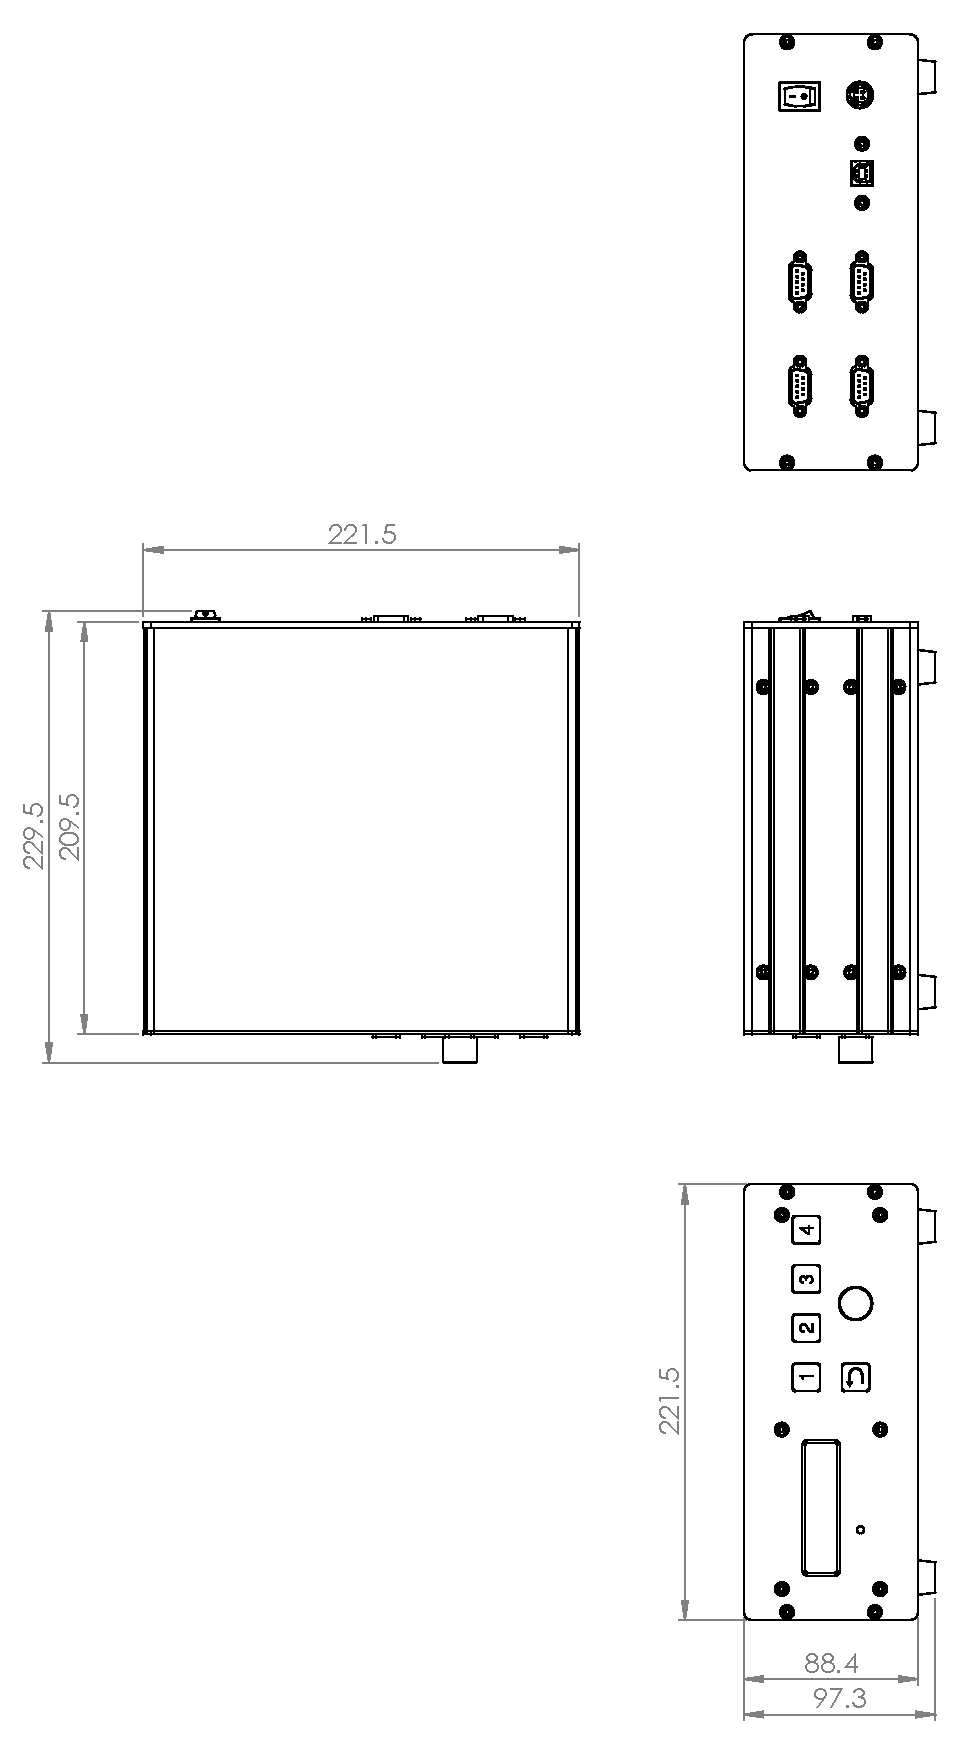
\includegraphics[angle=0,origin=c,width=0.7\textwidth]{./drawings/MG22131_outline2.pdf}
\end{figure}
%\vfill
\FloatBarrier

\subsection*{Pin Configuration}
\begin{minipage}{\textwidth}
  \begin{minipage}[b]{0.49\textwidth}
    \centering
    D-SUB-9 female connector\\
    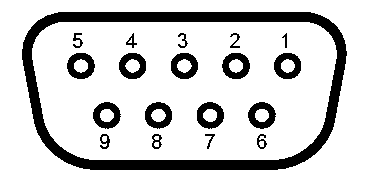
\includegraphics[width=0.6\textwidth]{./drawings/Numbered_DE9_female_Diagram.pdf}\\
    Front view
  \end{minipage}
  \hfill
  \begin{minipage}[b]{0.49\textwidth}
    \centering
    \begin{tabular}{cc}
      \toprule
      \textbf{Pin} & \textbf{Function} \\
      \toprule
      1 & Phase B1 \\ \midrule
      2 & Phase B2\\ \midrule
      3 & Phase A2 \\ \midrule
      4 & Phase A1 \\ \midrule
      5 & Ground \\ \midrule
      6 & +5V \\ \midrule
      7 & Sens 1 \\ \midrule
      8 & Sens 2 \\ \midrule
      9 & Sens 3 \\ \midrule
      Shield & NC \\
      \bottomrule
    \end{tabular}
  \end{minipage}
\end{minipage}
\FloatBarrier

\subsection*{Ordering Information}

\tikzstyle{every node}=[anchor=west,align=left]
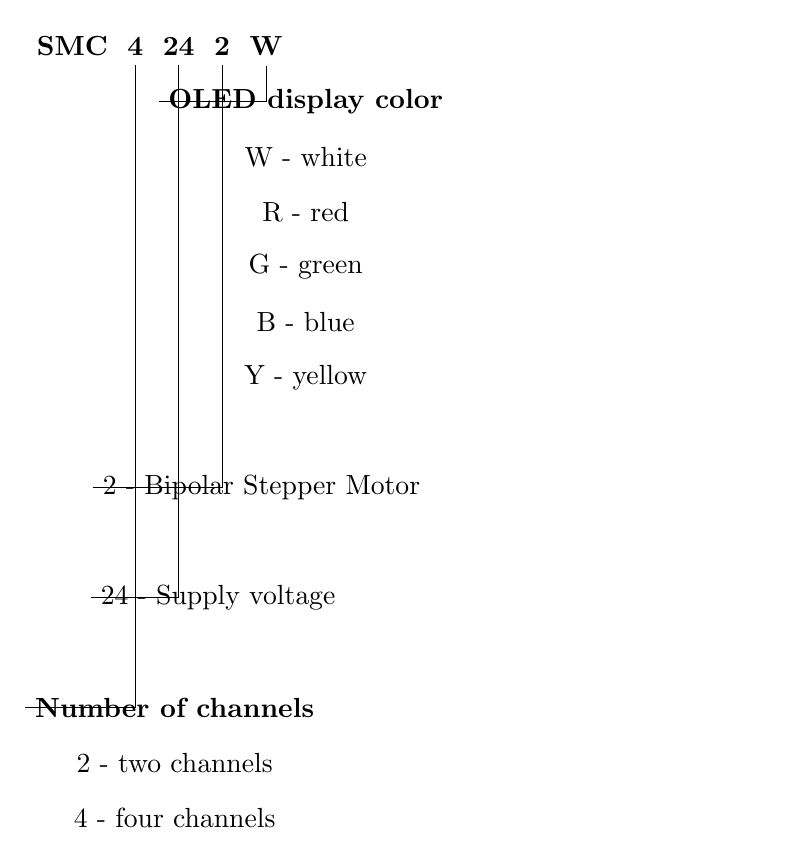
\begin{tikzpicture}[
  grow via three points={one child at (0.5,-0.7) and
  two children at (0.5,-0.7) and (0.5,-1.4)},
  edge from parent path={(\tikzparentnode.south) |- (\tikzchildnode.west)}]
  \node (SMC) {\textbf{SMC}};
  \hspace{-10mm}
  \node (motors) [right= of SMC] {\textbf{4}}
    child [missing] {}
    child [missing] {}
    child [missing] {}
    child [missing] {}
    child [missing] {}
    child [missing] {}
    child [missing] {}
    child [missing] {}
    child [missing] {}
    child [missing] {}
    child [missing] {}
    child { node {\textbf{Number of channels}}}
    child { node {2 - two channels} edge from parent[draw=none] }
    child { node {4 - four channels} edge from parent[draw=none] };
  \hspace{-10mm}
  \node (voltage) [right= of motors] {\textbf{24}}
    child [missing] {}
    child [missing] {}
    child [missing] {}
    child [missing] {}
    child [missing] {}
    child [missing] {}
    child [missing] {}
    child [missing] {}
    child [missing] {}
    child { node {24 - Supply voltage}};
  \hspace{-10mm}
  \node (motorType) [right= of voltage] {\textbf{2}}
    child [missing] {}
    child [missing] {}
    child [missing] {}
    child [missing] {}
    child [missing] {}
    child [missing] {}
    child [missing] {}
    child { node {2 - Bipolar Stepper Motor}};
  \hspace{-10mm}
  \node (color) [right= of motorType] {\textbf{W}}
    child { node {\textbf{OLED display color}}}		
    child { node {W - white} edge from parent[draw=none] }
    child { node {R - red} edge from parent[draw=none] }
    child { node {G - green} edge from parent[draw=none] }
    child { node {B - blue} edge from parent[draw=none] }
    child { node {Y - yellow} edge from parent[draw=none] };
\end{tikzpicture}






\FloatBarrier
\vfill
\end{document}
